% Canonical source for the Parallage preprint.
% Build from the repository root with `make`; XeLaTeX is required.
%
% Options for packages loaded elsewhere
\PassOptionsToPackage{unicode}{hyperref}
\PassOptionsToPackage{hyphens}{url}
\PassOptionsToPackage{dvipsnames,svgnames,x11names}{xcolor}
%
\documentclass[
  12pt,
]{article}
\usepackage{amsmath,amssymb}
\usepackage{setspace}
\usepackage{iftex}
\ifPDFTeX
  \usepackage[T1]{fontenc}
  \usepackage[utf8]{inputenc}
  \usepackage{textcomp} % provide euro and other symbols
\else % if luatex or xetex
  \usepackage{unicode-math} % this also loads fontspec
  \defaultfontfeatures{Scale=MatchLowercase}
  \defaultfontfeatures[\rmfamily]{Ligatures=TeX,Scale=1}
\fi
\usepackage{lmodern}
\ifPDFTeX\else
  % xetex/luatex font selection
\fi
% Use upquote if available, for straight quotes in verbatim environments
\IfFileExists{upquote.sty}{\usepackage{upquote}}{}
\IfFileExists{microtype.sty}{% use microtype if available
  \usepackage[]{microtype}
  \UseMicrotypeSet[protrusion]{basicmath} % disable protrusion for tt fonts
}{}
\makeatletter
\@ifundefined{KOMAClassName}{% if non-KOMA class
  \IfFileExists{parskip.sty}{%
    \usepackage{parskip}
  }{% else
    \setlength{\parindent}{0pt}
    \setlength{\parskip}{6pt plus 2pt minus 1pt}}
}{% if KOMA class
  \KOMAoptions{parskip=half}}
\makeatother
\usepackage{xcolor}
\usepackage[margin=1in]{geometry}
\usepackage{longtable,booktabs,array}
\usepackage{pdflscape}
\usepackage{calc} % for calculating minipage widths
% Correct order of tables after \paragraph or \subparagraph
\usepackage{etoolbox}
\makeatletter
\patchcmd\longtable{\par}{\if@noskipsec\mbox{}\fi\par}{}{}
\makeatother
% Allow footnotes in longtable head/foot
\IfFileExists{footnotehyper.sty}{\usepackage{footnotehyper}}{\usepackage{footnote}}
\makesavenoteenv{longtable}
\usepackage{graphicx}
\makeatletter
\def\maxwidth{\ifdim\Gin@nat@width>\linewidth\linewidth\else\Gin@nat@width\fi}
\def\maxheight{\ifdim\Gin@nat@height>\textheight\textheight\else\Gin@nat@height\fi}
\makeatother
% Scale images if necessary, so that they will not overflow the page
% margins by default, and it is still possible to overwrite the defaults
% using explicit options in \includegraphics[width, height, ...]{}
\setkeys{Gin}{width=\maxwidth,height=\maxheight,keepaspectratio}
% Set default figure placement to htbp
\makeatletter
\def\fps@figure{htbp}
\makeatother
\setlength{\emergencystretch}{3em} % prevent overfull lines
\providecommand{\tightlist}{%
  \setlength{\itemsep}{0pt}\setlength{\parskip}{0pt}}
\setcounter{secnumdepth}{-\maxdimen} % remove section numbering
\usepackage{fontspec}
\usepackage{xeCJK}
\setmainfont{FreeSerif.otf}[
  BoldFont=FreeSerifBold.otf,
  ItalicFont=FreeSerifItalic.otf,
  BoldItalicFont=FreeSerifBoldItalic.otf
]
\setCJKmainfont{HaranoAjiMincho-Regular.otf}[
  BoldFont=HaranoAjiMincho-Bold.otf,
  ItalicFont=HaranoAjiMincho-Regular.otf
]
\setCJKmonofont{HaranoAjiGothic-Regular.otf}
\widowpenalty=10000
\clubpenalty=10000
\displaywidowpenalty=10000
\ifLuaTeX
  \usepackage{selnolig}  % disable illegal ligatures
\fi
\usepackage{bookmark}
\IfFileExists{xurl.sty}{\usepackage{xurl}}{} % add URL line breaks if available
\urlstyle{same}
\hypersetup{
  pdftitle={Parallage: Structured Alternatives for Auditing AI Translations of Ancient Texts},
  pdfauthor={Greg Baker; Shirley Chan; Vanessa Enriquez Raido; Greta Hawes},
  colorlinks=true,
  linkcolor={Maroon},
  filecolor={Maroon},
  citecolor={Blue},
  urlcolor={Blue},
  pdfcreator={XeLaTeX}}

\title{Parallage: Structured Alternatives for Auditing AI Translations
of Ancient Texts}
\author{Greg Baker \and Shirley Chan \and Vanessa Enriquez
Raido \and Greta Hawes}
\date{Preprint, 27 July 2026}

\begin{document}
\maketitle

\setstretch{1.08}
\section{Abstract}\label{abstract}

Large language models make it inexpensive to generate many translations,
including for ancient and under-translated texts, but they do not make
those translations easy to verify. A single fluent output can conceal
ambiguity, unstable named entities, and interpretive decisions from
readers who cannot inspect the source language. We introduce
\textbf{Parallage}, a human-facing method that presents a focal
translation with deliberately differentiated helper variants and
lightweight audit scaffolding. Unlike n-best reranking,
minimum-Bayes-risk decoding, or self-consistency, Parallage does not
collapse its candidate set into one answer or treat agreement among
correlated outputs as independent corroboration. It preserves structured
variation as an object for inspection.

We implement the method for Ancient Greek and Classical Chinese, release
a versioned library of twenty-seven helper profiles, and define an
anticipated-divergence judgement that can be elicited before an expert
reference is revealed. Formative co-author reviews show both possible
signal and serious confounding. In Greek, one reviewer's ratings track
the focal translation's XCOMET-XL divergence from the hidden human
rendering strongly (Spearman rho = 0.80, exact two-sided p = 0.008),
which taken alone would read as a successful pilot. But XCOMET
similarity falls steeply with passage length in this corpus, the same
ratings rise with length, and controlling for length attenuates the
association (partial rank r = 0.51, p = 0.130): a reader could have
scored almost as well by distrusting long passages. In ten Chinese
passages, where scores are not length-patterned, anticipated divergence
correlates modestly with an eight-metric reference-divergence composite
(Spearman rho = 0.47, exact one-sided p = 0.085) and most strongly with
XCOMET-XL (rho = -0.73, exact two-sided p = 0.020). The
five-pack/five-single Chinese split is too small and order-confounded to
estimate a treatment effect, and timing instrumentation failed in the
single-output condition. We therefore make no efficacy claim. The
contribution is a reproducible way to generate and expose translation
multiplicity, an auditable pilot with its confounds documented, and a
controlled-study protocol for testing whether structured alternatives
improve issue detection and confidence calibration.

\section{1. Abundant Translation, Scarce
Verification}\label{abundant-translation-scarce-verification}

Generative AI can produce fluent but incorrect translations quickly and
cheaply, making it attractive for fragmentary, specialised, or
under-translated ancient texts. The economics are stark: professional
human translation is conventionally budgeted at roughly
\$0.10--\$0.15 per source word, while generating this project's full
set of twenty-seven helper renderings cost about 0.7 cents per source
word, and web dissemination costs almost nothing. The failures of
generated translation, however, can be concentrated rather
than gradual. In a reference-free expert evaluation of Ancient Greek
technical prose, Zainaldin et al.~(2026) found high average performance
but catastrophic failures on two terminology-dense passages, with
terminology rarity the dominant predictor of failure. Standard automatic
metrics were informative only when the candidate set contained wide
quality variation. This combination---mostly fluent output, sparse
severe failures, and incomplete metric discrimination---makes
verification a retrieval problem as well as a translation problem:
limited expert attention must be directed to the passages and decisions
most likely to need it.

The verification problem is especially acute when no stable complete
translation exists. Readers of New Testament Greek can triangulate with
dictionaries, parallel translations, and extensive commentary. Readers
of Stephanos of Byzantium's \emph{Ethnica} or the Tsinghua bamboo
manuscript \emph{Xin shi wei zhong} often cannot: no complete prior
English translation exists, the author cannot be asked what they meant,
and no native speaker raised in the source culture survives to consult.
A non-reader of Greek
or Classical Chinese cannot independently inspect the source script. If
one of the translations sounds fluent, how can they tell if there are
problems?

The central question is not whether a candidate can be made to look
reliable, but whether a reader can be given useful evidence about where
it may not be. The design premise is deliberately inverted from
conventional translation delivery: rather than trying to remove
ambiguity and uncertainty, Parallage tries to make them obvious. It uses
a set of role-conditioned translations for
that purpose. The outputs are not votes, and the most fluent or central
output is not automatically selected as correct. The set is presented to
a person who must decide where to distrust, investigate, or seek expert
help.

This paper makes four contributions:

\begin{enumerate}
\def\labelenumi{\arabic{enumi}.}
\tightlist
\item
  A reproducible parallel-pack method with one focal translation,
  twenty-seven versioned helper profiles, and generation provenance.
\item
  A cross-script pilot over Ancient Greek and Classical Chinese.
\item
  An anticipated-divergence instrument that non-readers can answer and
  later compare with an independent human rendering.
\item
  An evidence-led protocol for a preregistered controlled study of
  whether packs improve issue detection and confidence calibration.
\end{enumerate}

\section{2. Related Work}\label{related-work}

\subsection{2.1 Multiple Hypotheses in Machine
Translation}\label{multiple-hypotheses-in-machine-translation}

Machine-translation systems have long generated candidate lists,
lattices, or samples. Most computational uses of this multiplicity are
decision procedures. Minimum-Bayes-risk decoding, for example, selects
the candidate with the best expected utility under a model and metric
rather than exposing the candidate set to a reader (Freitag et
al.~2022). Multi-hypothesis evaluation instead uses diverse translations
to model reference variation or quantify system uncertainty (Fomicheva,
Specia, and Guzmán 2020). Parallage shares the premise that one
reference and one output hide legitimate variation, but assigns
multiplicity a different role: the variants are contrastive evidence in
a user interface.

This difference matters because candidate agreement is not a calibrated
confidence estimate. Twenty-seven outputs from the same model family,
prompted by related instructions and trained on overlapping data, are
not twenty-seven independent witnesses. A shared error can appear stable
across the pack. Conversely, deliberate style changes can produce
surface disagreement without any underlying semantic dispute. Parallage
therefore uses role diversity to elicit inspectable decisions, not
majority voting.

\subsection{2.2 Quality Estimation and Human
Reliance}\label{quality-estimation-and-human-reliance}

Reference-free quality estimation aims to predict translation quality
when no human reference is available. Learned metrics can help locate
errors, but quality scores do not by themselves determine how a person
should rely on a translation. In a clinical study, Mehandru et
al.~(2023) found that quality-estimation feedback and back-translation
affected different aspects of physicians' reliance decisions,
illustrating the need to evaluate decision support in its context of
use. Work on neural-MT hallucination detection likewise finds that
fluent critical errors are rare and difficult to identify, and that
commonly used detectors can fail in preventive settings (Guerreiro,
Voita, and Martins 2023).

Parallage is complementary to quality estimation. It does not require a
calibrated score at reading time, although scores and expert references
can be used later to evaluate judgements. Its main object is the human
decision: which spans or passages should be distrusted, and with what
confidence?

\subsection{2.3 Sampling-Based
Self-Checking}\label{sampling-based-self-checking}

Self-consistency, multi-agent debate, semantic entropy, and black-box
self-checking generate multiple model outputs to select an answer or
estimate uncertainty (Wang et al.~2023; Du et al.~2024; Farquhar et
al.~2024; Manakul, Liusie, and Gales 2023). These approaches motivate
using variation as evidence, while also exposing a limit relevant here:
agreement can be uninformative when outputs are systematically wrong.
Parallage moves the evidence boundary outward. Instead of using sampled
variation only inside the system, it gives deliberately structured
variation to the reader and measures the reader's subsequent judgement.

\section{3. The Parallage Method}\label{the-parallage-method}

\emph{Parallage} draws on Greek παραλλαγή, variation or alternation. A
parallel translation pack contains three layers:

\begin{enumerate}
\def\labelenumi{\arabic{enumi}.}
\tightlist
\item
  A \textbf{focal translation}, representing the single fluent rendering
  at which a conventional interface might stop.
\item
  \textbf{Helper variants}, generated under systematically different
  prompt profiles rather than by repeatedly sampling one prompt.
\item
  \textbf{Audit scaffolding}, including source-segment alignment,
  named-entity handling, marked ambiguity points, disagreement cues, and
  review prompts.
\end{enumerate}

The current implementation has one focal profile and twenty-seven helper
profiles. The helper count is the ``twenty-seven prompts'' described in
the associated talk; including the focal profile gives twenty-eight
generated outputs per passage in the Chinese analysis. The profiles fall
into four functional families:

\begin{longtable}[]{@{}
  >{\raggedright\arraybackslash}p{(\columnwidth - 4\tabcolsep) * \real{0.3333}}
  >{\raggedright\arraybackslash}p{(\columnwidth - 4\tabcolsep) * \real{0.3333}}
  >{\raggedright\arraybackslash}p{(\columnwidth - 4\tabcolsep) * \real{0.3333}}@{}}
\toprule\noalign{}
\begin{minipage}[b]{\linewidth}\raggedright
Family
\end{minipage} & \begin{minipage}[b]{\linewidth}\raggedright
Example profiles
\end{minipage} & \begin{minipage}[b]{\linewidth}\raggedright
Intended inspection function
\end{minipage} \\
\midrule\noalign{}
\endhead
\bottomrule\noalign{}
\endlastfoot
Philological & diplomatic literal, interlinear gloss, syntax scaffold,
minimal inference & expose source structure and supplied inference \\
Reader-facing & scholarly readable, smooth idiomatic, controlled
English, plain language & contrast editorial smoothing and accessibility
choices \\
Analytical & entity explicit, forked lattice, uncertainty annotated,
decision log, adversarial, back-translation audit & surface entities,
forks, confidence claims, drift, and possible counter-readings \\
Creative/mnemonic & mnemonic, alliterative, rhyming & stress lexical
choices under strong form constraints; not candidate critical
translations \\
\end{longtable}

These roles are hypotheses about useful forms of multiplicity, not a
claim that all twenty-seven helpers are necessary. Several profiles
produce apparatus as well as translation text, and some ``pack''
profiles deliberately combine related functions. The controlled study
will log which components readers actually use so that later versions
can remove redundant or distracting roles.

\begin{figure}
\centering
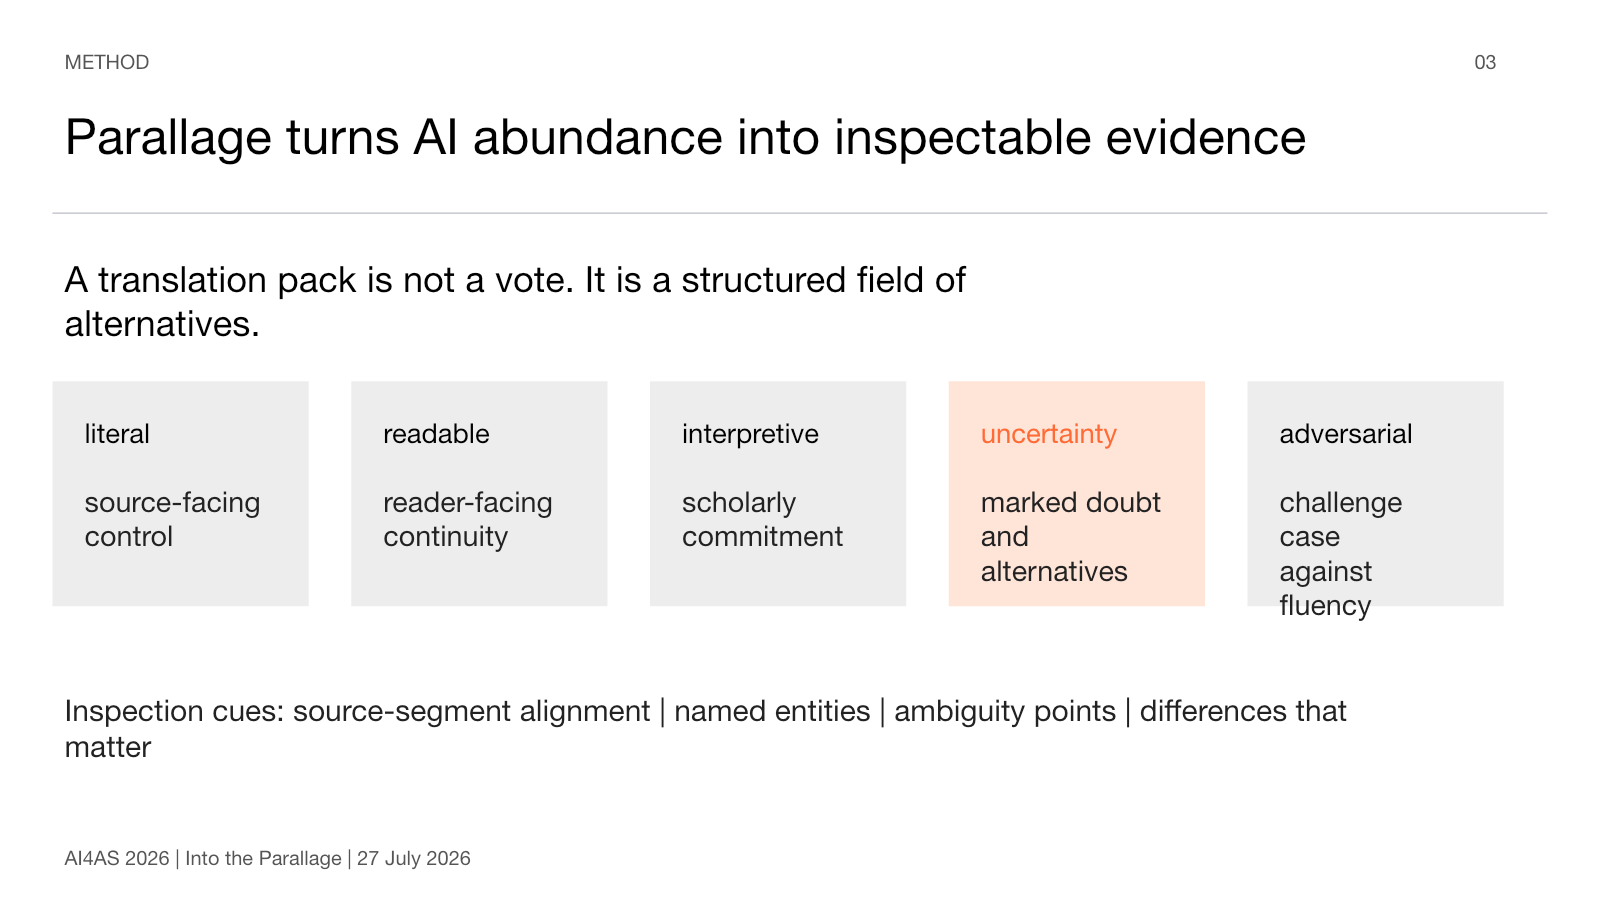
\includegraphics[width=1\textwidth,height=\textheight]{figures/parallage-pack-schematic.png}
\caption{Schematic of the core Parallage pack roles and inspection cues.
A pack presents structured alternatives rather than treating the
variants as a vote.}
\end{figure}

Agreement across variants is a cue to inspect, not proof. Outputs
produced by related models and prompts are correlated and may repeat the
same error. Disagreement is likewise a cue rather than a guarantee that
one variant is correct. The method's claim is therefore narrower than
ensemble corroboration: contrasting renderings can expose decisions that
a single fluent output concealed.

\subsection{3.1 A Worked Crux: the Graph
麏}\label{a-worked-crux-the-graph-jun}

Chinese passage 7 reads:

\begin{quote}
寧心謀之、稽之、度之、鑒之，聞訊視聽，在善之麏，心焉為之。\\
\emph{Níng xīn móu zhī, jī zhī, duó zhī, jiàn zhī; wén xùn shì tīng,
zài shàn zhī jūn; xīn yān wéi zhī.}
\end{quote}

The phrase 在善之麏 is genuinely difficult. The graph 麏 ordinarily
denotes a deer; here it may stand for a herd, cluster, or gathering,
and scholars generally read it as 攈, ``to gather, glean''. The focal
translation keeps the animal image, rendering the phrase ``amid the
gathered `herd' of what is good''---fluent, and silent about the
problem. The helpers are not silent: twenty-two of the twenty-seven
helper profiles mark the graph as uncertain somewhere in their output.
The scholarly-readable profile translates cautiously and then flags the
crux in its glossary:

\begin{quote}
善之麏: uncertain. 麏 may suggest a ``herd/cluster/gathering,'' so
translated cautiously as ``the gathered forms of what is good.''
\end{quote}

Even the rhyming profile, built for play rather than criticism, is
forced to disclose the unresolved choice in its final line:

\begin{quote}
Calm the heart: devise it, search it, weigh its way;\\
Hold it to the mirror's light by day.\\
Hear, question, look, and listen where you should;\\
The heart acts there---among the herd/deer? of good.
\end{quote}

The rhyme is not a candidate critical translation. Its usefulness is
diagnostic: the pressure to complete the rhyme makes the unresolved
lexical choice impossible to miss. A reader might pass over the odd
herd image in the focal translation alone; against the pack, the
problem is unmissable. Shirley Chan's expert reference translation,
recorded after the pilot review, resolves the crux with the gather
reading: ``The tranquil heart-mind deliberates on it, examines it,
measures it, and reflects on it. In hearing, questioning, looking and
listening, lies within the gathered goodness (for which) the heart-mind
thereby acts for it.''

The pack helps with smaller decisions in the same passage. Most
profiles render 寧心 as an imperative (``calm the mind'', ``settle the
heart-mind''), while the forked-lattice and decision-log profiles
record ``with a tranquil mind'' as a live alternative---a fork that a
single fluent output would have closed silently.

\section{4. Corpora and
Implementation}\label{corpora-and-implementation}

\subsection{4.1 Ancient Greek}\label{ancient-greek}

The Greek corpus uses entries from Stephanos of Byzantium's
\emph{Ethnica}, a late-antique geographical lexicon and arguably the
oldest surviving alphabetically organised encyclopedic work---earlier
alphabetical compilations are word-glossaries, and the \emph{Suda} is
four centuries later---preserved incompletely and without a complete
published English translation
(Meineke 1849; Billerbeck 2006-present). From a pool of 100 entries with
approved human translations, we drew a reproducible seeded sample of
twenty (seed 20260623). The entries are compressed, entity-heavy, and
varied in length. The project's automated scholarly rendering is the
focal translation; the approved human translation is hidden during
review.

Model-development results provide context for why inspection remains
necessary. A companion operational benchmark contains 100 Kappa entries,
each with one approved project translation, crossed with twelve dated
OpenAI releases and three prompt conditions. The minimal condition
simply asks the model to act as a classical translator. The reviewed
prompt was written by Anthropic's Claude when shown twenty
project-corrected translations alongside the model's earlier attempts,
and encodes recurring constructions, named-entity handling, and
editorial conventions. The detailed condition is its later, more
modular revision, supplying guidance only for constructions present in
an entry, and is the basis of the Greek focal profile (Section 4.3).
Twenty prompt-development entries remain inside the benchmark, so these
are retrospective measurements of the project workflow rather than
scores on an untouched test set. Across the resulting 3,600
model-entry comparisons, the mean of BLEU-4, chrF++, METEOR, and ROUGE-L
(Papineni et al.~2002; Popović 2017; Banerjee and Lavie 2005; Lin 2004)
rose from 43.0\% to 47.2\% under a minimal prompt, from 60.9\% to 70.0\%
under a reviewed prompt, and from 58.9\% to 72.9\% under a detailed
prompt-plus-guidance workflow: gains of 4.2, 9.1, and 14.0 percentage
points. Even the strongest 2026 cell remains more than eleven points
below the 84.3\% mean overlap of retained expert first drafts against
their approved revisions, so expert verification remains binding under
every prompt condition.

\begin{figure}
\centering
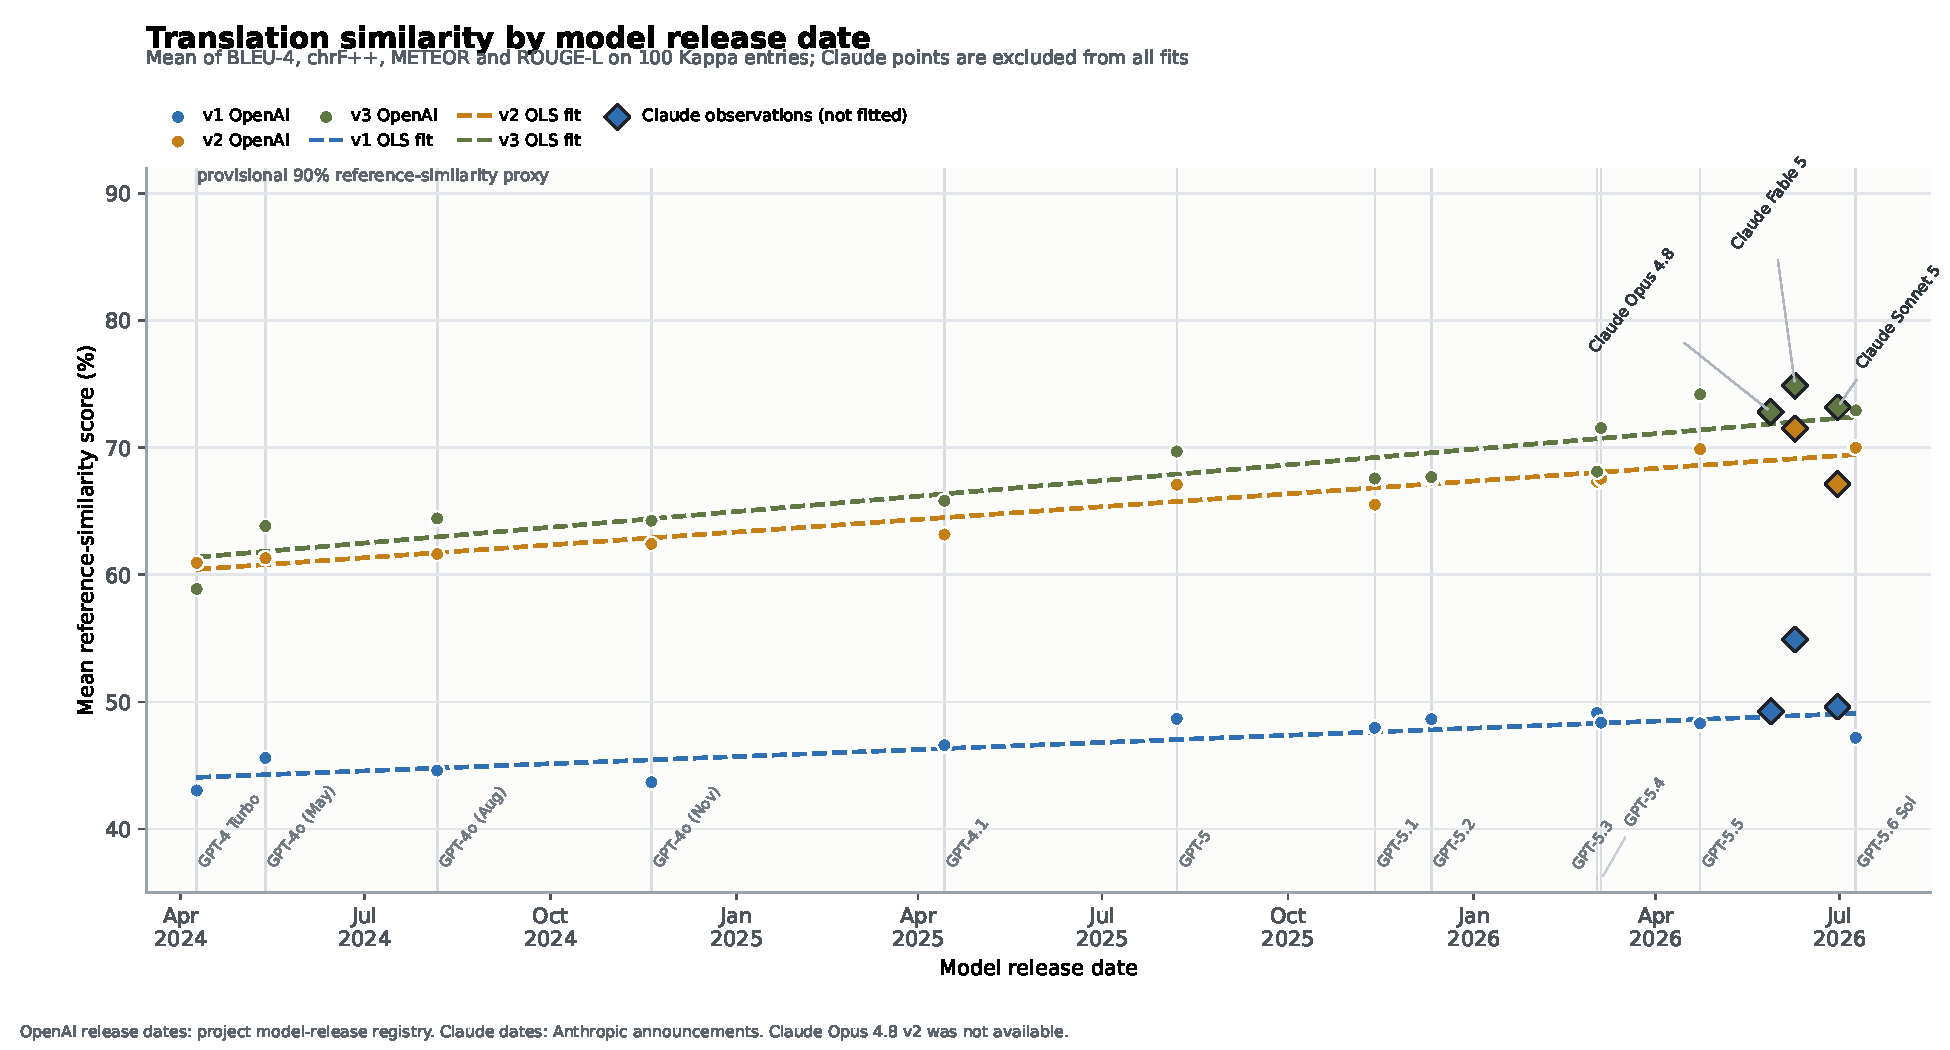
\includegraphics[width=1\textwidth,height=\textheight]{figures/model-quality-over-time.pdf}
\caption{Mean four-metric reference similarity on the 100-entry Kappa
benchmark by model release date under the three prompt conditions, with
ordinary least-squares fits. Anthropic Claude observations are plotted
for context and excluded from the fits. The dotted line is a provisional
90\% reference-similarity proxy; no fitted trend crosses it before
2030.}
\end{figure}

Ordinary least-squares fits of the per-release means against release
date give slopes of 2.2, 4.0, and 4.9 percentage points per year for the
minimal, reviewed, and detailed conditions (R\textsuperscript{2} = 0.71,
0.93, and 0.82). Extrapolated naively, the detailed workflow does not
reach the 84.3\% draft-overlap bar until about 2029 and the provisional
90\% proxy until 2030; the reviewed prompt crosses the same bars around
2030 and 2032; the minimal prompt would take until the 2040s. These
extrapolations illustrate a verification horizon; they are not
forecasts. The scores are within-project reference similarities rather
than calibrated measures of philological correctness or human
equivalence, the linear trend may saturate or jump, and crossing a
similarity bar is necessary rather than sufficient for expert-quality
translation. Nor does the literature supply a single number for
``human-level'' reference similarity: in the original BLEU evaluation a
human translator scored 0.26 against two other human references and
0.35 against four (Papineni et al.~2002), and standard references
concentrate around translationese, penalising legitimate alternative
renderings (Freitag, Grangier, and Caswell 2020). Both bars used here
are within-workflow yardsticks---the draft-overlap bar shares a
translator and house conventions, and the 90\% proxy is an illustration
rather than a measured inter-translator ceiling. What survives those caveats is operational: unless
capability growth breaks from its current trend, expert verification
remains essential for ancient-language translation for the remainder of
this decade at least, and prompt specification alone moves that horizon
by years.

XCOMET-XL, a learned metric combining sentence scoring with error-span
detection, gives a direct within-workflow calibration (Guerreiro et
al.~2024). Seventy-nine retained initial expert drafts score 0.5741 on
average against their approved revisions (95\% CI 0.5213-0.6270). On
those same entries GPT-5.6 scores 0.5944 under the reviewed prompt and
0.6013 under the detailed prompt. The paired model-minus-draft
difference is inconclusive for the reviewed prompt (0.0203, p=0.087) and
small but positive for the detailed prompt (0.0272, p=0.023). On this
metric, the current production workflow has reached the reference
similarity of the retained pre-review drafts. It does not
establish human parity: the human comparison is a draft before expert
review, the approved version is the scoring reference, and the prompts
encode conventions learned during the same editorial process.

\subsection{4.2 Classical Chinese}\label{classical-chinese}

The Chinese corpus is \emph{Xin shi wei zhong} 心是謂中, a Warring
States bamboo manuscript published in volume 8 of the Tsinghua
collection (Shen 2018). The manuscript concerns the heart-mind (xin
心), deliberation, and ethical judgement. The two corpora were chosen
to differ: where the \emph{Ethnica} is concrete, cataloguing particular
places and peoples, \emph{Xin shi wei zhong} is abstract and
philosophical, equally compressed in syntax, and adds
textual-reconstruction problems of its own. Shirley
Chan supplied the project working
transcription and approved a ten-part segmentation in July 2026. After
Greta's anticipated-divergence review had been completed, Shirley
supplied an English reference translation for each of the ten passages.
These references are recorded as the Chinese ground-truth set in the
analysis database, but we treat them in the paper as expert reference
translations rather than as uniquely correct renderings.

If Parallage works across both traditions, it is a candidate general
method; if it works in only one, disciplinary design must remain local.

\subsection{4.3 Generation and Review
Infrastructure}\label{generation-and-review-infrastructure}

All focal and helper translations used in the review interface were
generated with \texttt{gpt-5.5}. The Greek focal translation used
version 3 of the project's reviewed scholarly profile; the Chinese focal
profile requested one clear scholarly translation without commentary, a
minimal instruction comparable to the benchmark's minimal condition, so
the Chinese focal translations should be expected to carry more errors
than the prompt-engineered Greek ones.
The twenty-seven helper profiles were version 1. For Chinese, each of
the ten passages was generated once under each profile through the
Responses API with a maximum of 2,400 output tokens. Temperature and
seed were not supplied, so the stored outputs are reproducible as
versioned artifacts rather than as deterministic regenerations. Each
record stores passage, profile and version, model, run identifier,
status, output text, response identifier, usage metadata, and completion
time.

The Chinese assignment was created with seed 20260704. Five passages
were assigned to show the focal translation plus all available helpers
and five to show the focal translation alone; display order was also
seeded. This is a within-reviewer pilot assignment, not
participant-level randomisation. The Greek review set used a
twenty-entry sample drawn with Python's
\texttt{random.Random(seed).sample} from the sorted pool of entries with
approved human translations (seed 20260623). Reviewers completed
overlapping subsets rather than a controlled interface comparison.

The browser interface logs each saved rating and an exposure record for
helper cards entering the tracked viewport. Viewport exposure is an
interaction trace, not proof that a card was read. The database keeps
focal and helper run identifiers, prompt versions, treatment assignment,
display order, and later expert-reference records separately. Human
attention and expert adjudication, rather than model generation, remain
the limiting resources.

\section{5. Pilot Method}\label{pilot-method}

\subsection{5.1 Anticipated Divergence}\label{anticipated-divergence}

The review interface asks one question on an eleven-point scale:

\begin{quote}
How different would you expect the human translation to be to this
translation?\\
0 = will be the same; 10 = will be very different.
\end{quote}

\subsection{5.2 Reviewers, Materials, and
Analysis}\label{reviewers-materials-and-analysis}

The pilot observations came from three co-authors and internal
collaborators. Vanessa Enriquez Raido, a Translation Studies scholar,
reviewed ten Greek passages. Shirley Chan, a scholar of Chinese language
and culture, reviewed nineteen Greek passages. Nine passages overlap
between their sets. Greta Hawes, an ancient-world scholar who does not
read Classical Chinese, reviewed five Chinese passages with a full pack
and five with a single translation. Neither Vanessa nor Shirley reads
Ancient Greek, so every reviewer judged translations from a language
they could not read. These are formative co-design
observations, not an independent participant sample or evidence of
efficacy. Greg Baker developed the system and conducted the analysis but
did not contribute review ratings.

For the Greek passages we compared ratings with sentence-aligned BLEU-4
(Papineni et al.~2002), ROUGE-L (Lin 2004), character 3-gram F1, and
character 3-gram Jaccard against the approved human rendering, and with
XCOMET-XL scored on the same focal-reference pairs. Because the overlap
measures decline with reference length in the wider 101-translation
population, we fitted a per-metric log-length model and expressed each
observed score as residual badness: standard deviations worse than
expected for a passage of that length. We also report a composite of the
four residual measures and a population-standardised lexical ensemble,
the mean of the four per-metric z-scores against the same population.
Overlap-metric correlations are Spearman coefficients with asymptotic
two-sided p-values. XCOMET and ensemble correlations use permutation
tests instead: exact enumeration of the 151,200 unique orderings of
Vanessa's tied ratings, and a seeded 999,999-draw Monte Carlo
permutation for Shirley's nineteen. Length-controlled Greek estimates
are partial rank correlations between rating and XCOMET divergence given
log source length, with approximate p-values.

For Chinese, all 280 completed translations (twenty-eight profiles by
ten passages) were scored against Shirley's reference set using BLEU-4,
chrF++, METEOR, ROUGE-L, word unigram F1, word trigram F1, character
trigram F1, and word-edit similarity (Papineni et al.~2002; Popović
2017; Banerjee and Lavie 2005; Lin 2004). The ten focal translations
were additionally scored with BERTScore, COMET, XCOMET-XL, and BLEURT
(Zhang et al.~2020; Rei et al.~2020; Guerreiro et al.~2024; Sellam et
al.~2020). The primary divergence composite is the mean within-sample
badness percentile, scaled from 0 to 10, across BLEU-4, chrF++, METEOR,
ROUGE-L, BERTScore, COMET, XCOMET-XL, and BLEURT. It is a transparent
rank aggregate rather than a calibrated quality score.

The overall Chinese directional diagnostic asks whether a higher
anticipated-divergence rating predicts greater metric-derived
divergence; we report its exact one-sided permutation p-value over the
226,800 unique permutations of Greta's tied ratings. Individual-metric
and five-passage condition analyses use exact two-sided permutation
p-values. Pairwise ordering accuracy considers every comparable pair: a
pair is concordant when the passage Greta expects to differ more also
has greater composite divergence.

For the Chinese length diagnostic, source length is the number of
Han-script characters, avoiding an unvalidated word segmentation;
Shirley-reference word count is a sensitivity measure. We first
collapsed the balanced 280-row translation grid to ten passage means and
tested whether longer passages had lower mean lexical similarity. We
then fitted each of the eight focal primary metrics against log source
length, converted its negative residual to standardised badness, and
averaged the eight residuals. Unlike the Greek adjustment, these Chinese
length models are fitted on the same ten passages and therefore remain
exploratory.

The interface captured page-load-to-first-save latency. Later saves for
the same reviewer-passage pair were treated as revisions rather than
independent observations. Helper-card viewport time can overlap and does
not prove active reading.

All pilot analyses are exploratory and were performed after the
observations had been collected. Exact tests enumerate the unique
permutations of Greta's tied ratings. The directional composite test is
reported one-sided because the diagnostic asks whether greater
anticipated divergence predicts greater measured divergence;
metric-specific and condition-specific tests are two-sided. Confidence
intervals and effect estimates are emphasised because the sample sizes
are too small for stable threshold decisions.

\section{6. Formative Results}\label{formative-results}

\subsection{6.1 Judgement Signal and the Length
Confound}\label{judgement-signal-and-the-length-confound}

Judged against XCOMET-XL, the Greek pilot at first looks like a
success. Across her ten passages, Vanessa's ratings track the focal
translation's XCOMET divergence from the hidden human rendering at rho =
0.796 (exact two-sided p = 0.0085). Shirley's nineteen ratings trend the
same way but remain inconclusive (rho = 0.345, Monte Carlo p = 0.147).
Taken alone, the Vanessa association would usually be reported as a
successful experiment.

\begin{figure}
\centering
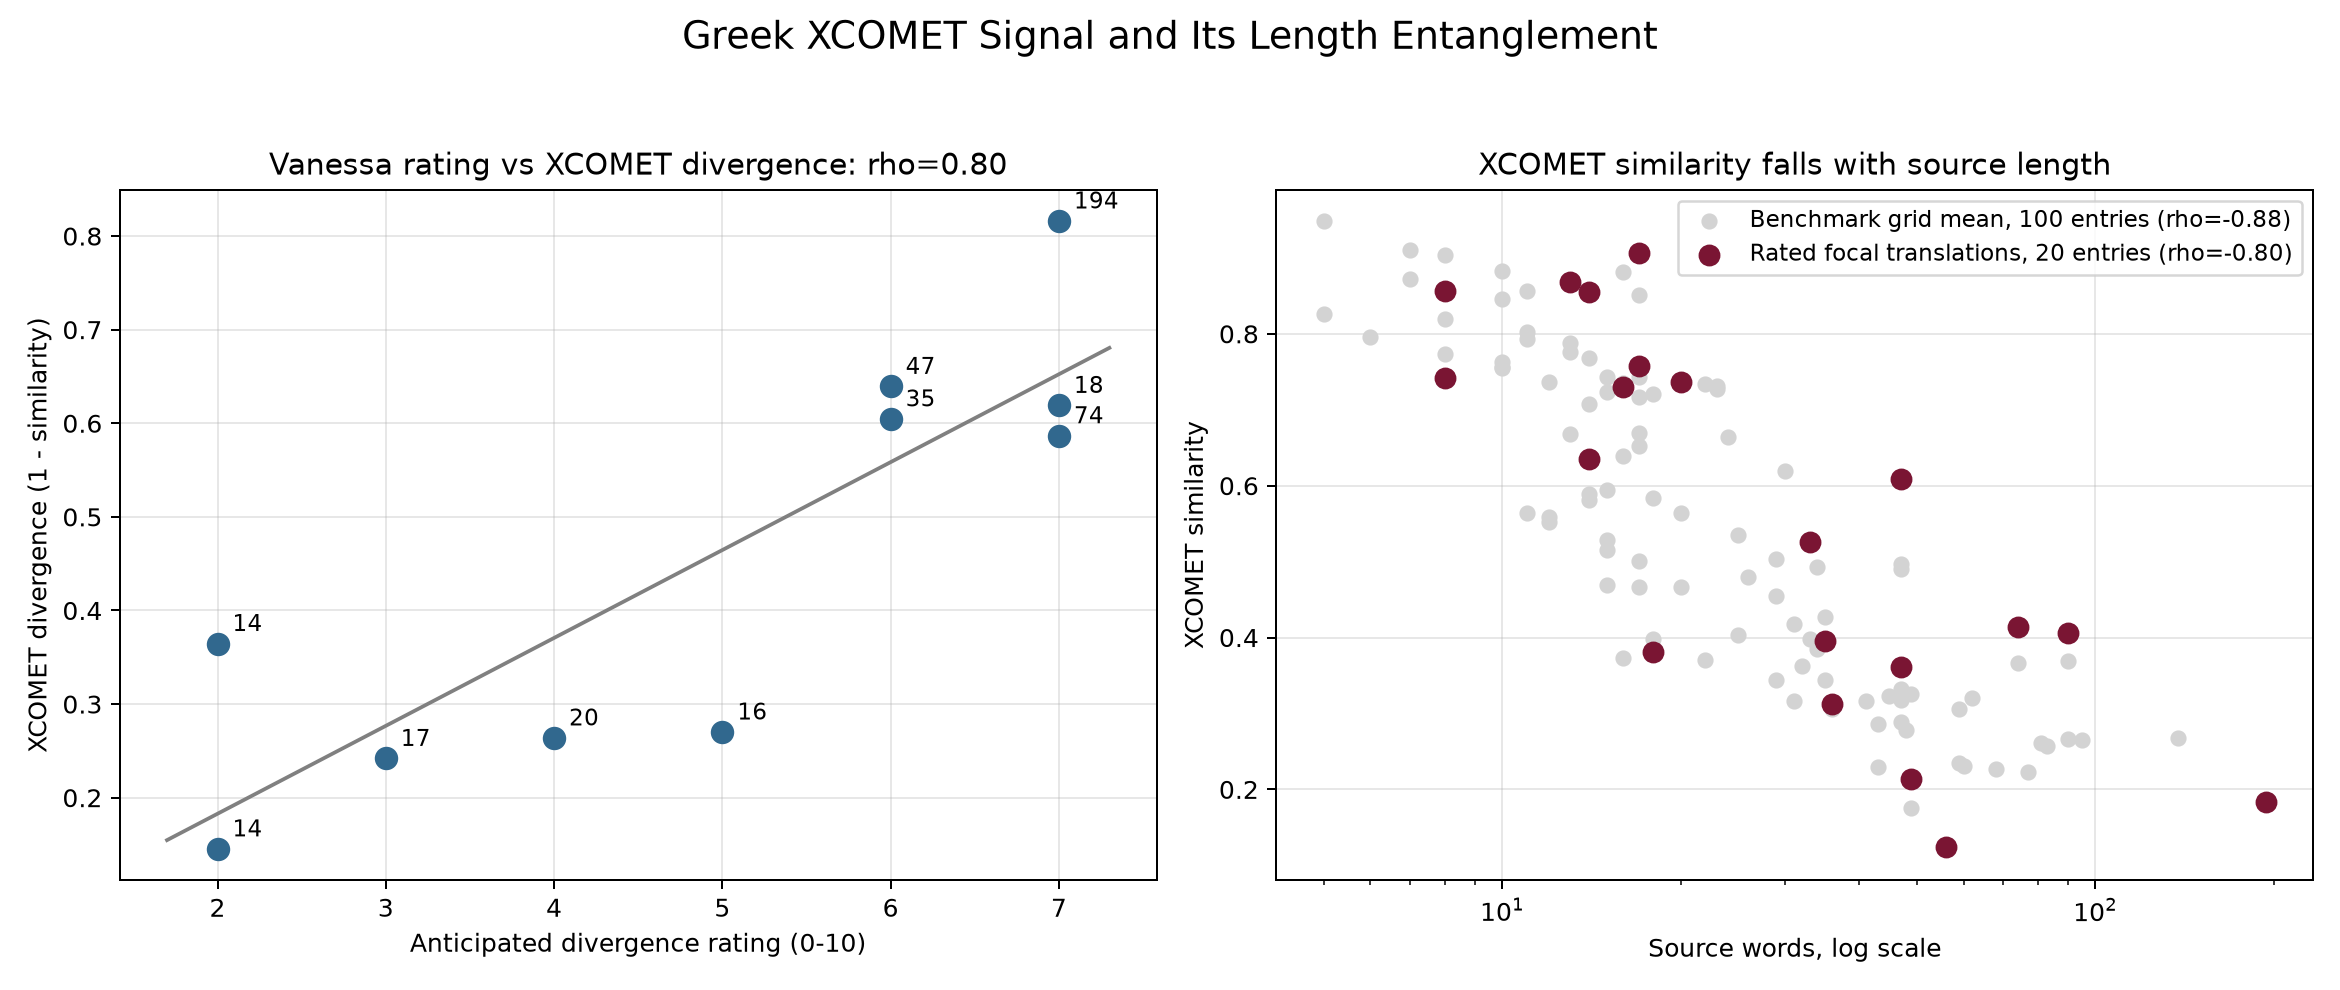
\includegraphics[width=1\textwidth,height=\textheight]{figures/greek-xcomet-confound.png}
\caption{Vanessa's anticipated-divergence ratings track XCOMET
divergence (left; point labels give source word counts), but XCOMET
similarity itself falls steeply with source length (right; grey points
are per-entry means across the companion benchmark grid, dark points the
twenty rated focal translations). A strong raw association is compatible
with a length heuristic.}
\end{figure}

The corpus embeds a confound that blocks that reading. Among the twenty
rated focal translations, XCOMET similarity falls steeply with source
length (rho = -0.80, p \textless{} 0.001), and the same gradient holds
across per-entry means of the companion benchmark grid (rho = -0.88 over
the same 100 entries). Vanessa's ratings in turn rise with reference
length (rho = 0.69, p = 0.027). A reader who understands neither the
source nor the target language could therefore score well on this
criterion simply by distrusting longer passages. Controlling for log
source length attenuates Vanessa's XCOMET association to a partial rank
correlation of 0.51 (p = 0.130); Shirley's becomes 0.19 (p = 0.43).
XCOMET was also selected for this comparison after inspection because it
was the strongest available measure; the overlap-metric results below
keep that selection visible.

The raw overlap-metric associations point in the expected direction, but
none is statistically significant. After adjustment for passage length,
the residual associations remain weak and inconclusive.

\begin{longtable}[]{@{}lrrrr@{}}
\toprule\noalign{}
Metric & Rating vs raw score & p & Rating vs residual badness & p \\
\midrule\noalign{}
\endhead
\bottomrule\noalign{}
\endlastfoot
BLEU-4 & -0.37 & 0.29 & 0.20 & 0.58 \\
ROUGE-L & -0.49 & 0.15 & 0.22 & 0.55 \\
3-gram F1 & -0.48 & 0.16 & 0.40 & 0.25 \\
3-gram Jaccard & -0.48 & 0.16 & 0.32 & 0.37 \\
\end{longtable}

The population-standardised lexical ensemble behaves the same way:
Vanessa's rating versus ensemble divergence is rho = 0.48 (exact p =
0.17), and versus composite length-adjusted badness only rho = 0.22 (p =
0.55). Shirley's ratings occupy a narrower 5-9 range; rating versus log
reference length is rho = 0.22 (p = 0.37), and rating versus composite
residual badness is rho = 0.13 (p = 0.60). Across the nine passages
rated by both reviewers, inter-reviewer association is moderate but
uncertain (rho = 0.44, p = 0.24).

The result is not that the pack works, and not that the reviewers
failed. It is that anticipated divergence is measurable, non-trivial,
and vulnerable to surface heuristics, and that a reference-based
criterion can reward those heuristics when the metric itself is
length-patterned. The controlled study must separate source difficulty,
passage length, lexical difference, and expert-adjudicated error.

\subsection{6.2 Chinese Reference-Based
Validation}\label{chinese-reference-based-validation}

Across all ten Chinese passages, Greta's anticipated-divergence rating
has a modest positive association with the eight-metric composite
divergence rank (Spearman rho = 0.472; exact one-sided p = 0.0848;
bootstrap 95\% interval -0.272 to 0.851). Kendall's tau is 0.303
(two-sided p = 0.237). Of the 41 passage pairs without a tied rating or
composite score, 27 are ordered correctly (65.9\%). Greta identifies two
of the three most divergent translations, but only one of the three
closest translations.

\begin{figure}
\centering
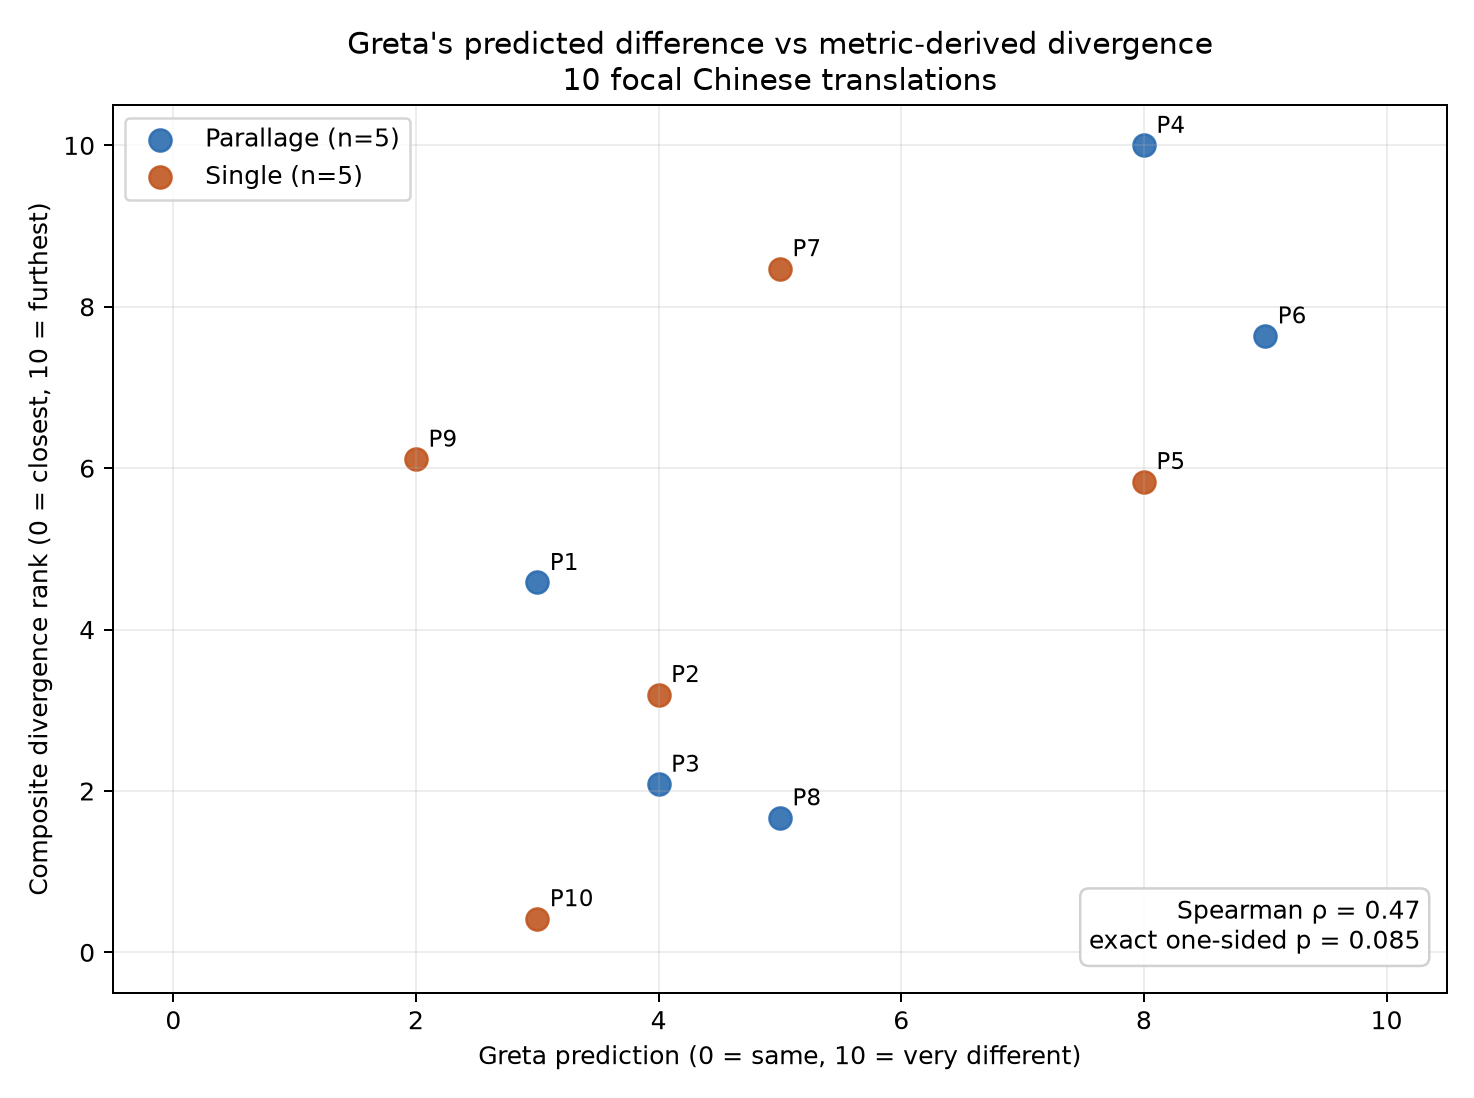
\includegraphics[width=1\textwidth,height=\textheight]{figures/chinese-prediction-scatter.png}
\caption{Greta's anticipated-divergence ratings against the eight-metric
composite for the ten focal Chinese translations. Colours show the
review condition, not independent samples.}
\end{figure}

The metric-level signs are consistent: higher predicted divergence
generally corresponds to lower reference similarity. XCOMET-XL gives the
strongest individual association (rho = -0.730, exact two-sided p =
0.0203). BLEURT is next strongest (rho = -0.626, p = 0.0584), while the
remaining metric estimates are directionally compatible but
statistically inconclusive. These twelve metrics are dependent measures
of the same ten translations. The XCOMET association is therefore a
promising convergence with one learned metric, not a confirmatory result
from twelve independent tests.

\begin{longtable}[]{@{}lrr@{}}
\toprule\noalign{}
Metric & Rating vs similarity rho & Exact p (two-sided) \\
\midrule\noalign{}
\endhead
\bottomrule\noalign{}
\endlastfoot
BLEU-4 & -0.417 & 0.2301 \\
chrF++ & -0.564 & 0.0936 \\
METEOR & -0.295 & 0.4067 \\
ROUGE-L & -0.337 & 0.3388 \\
Word unigram F1 & -0.393 & 0.2606 \\
Word trigram F1 & -0.540 & 0.1112 \\
Character trigram F1 & -0.564 & 0.0936 \\
Word-edit similarity & -0.522 & 0.1252 \\
BERTScore F1 & -0.399 & 0.2526 \\
COMET & -0.540 & 0.1112 \\
XCOMET-XL & -0.730 & 0.0203 \\
BLEURT & -0.626 & 0.0584 \\
\end{longtable}

The five-passage condition estimates do not distinguish the interface
treatments. Within the Parallage passages, composite rho is 0.500 (exact
two-sided p = 0.450); within the single-output passages it is 0.200 (p =
0.783). Each condition has six concordant and four discordant pairs,
hence the same 60\% pairwise ordering accuracy despite different
Spearman coefficients. Spearman correlation reflects the full rank
distances, whereas the pairwise measure counts only concordant versus
discordant orderings. For XCOMET, the five pack passages give rho =
-0.800 (exact p = 0.133) and the five single-output passages rho =
-0.600 (p = 0.350). The two estimates differ, but not by enough to
declare statistical significance with five passages per condition.

\begin{longtable}[]{@{}
  >{\raggedright\arraybackslash}p{(\columnwidth - 8\tabcolsep) * \real{0.1579}}
  >{\raggedleft\arraybackslash}p{(\columnwidth - 8\tabcolsep) * \real{0.2105}}
  >{\raggedleft\arraybackslash}p{(\columnwidth - 8\tabcolsep) * \real{0.2105}}
  >{\raggedleft\arraybackslash}p{(\columnwidth - 8\tabcolsep) * \real{0.2105}}
  >{\raggedleft\arraybackslash}p{(\columnwidth - 8\tabcolsep) * \real{0.2105}}@{}}
\toprule\noalign{}
\begin{minipage}[b]{\linewidth}\raggedright
Condition
\end{minipage} & \begin{minipage}[b]{\linewidth}\raggedleft
n
\end{minipage} & \begin{minipage}[b]{\linewidth}\raggedleft
Composite rho (exact p)
\end{minipage} & \begin{minipage}[b]{\linewidth}\raggedleft
XCOMET rho (exact p)
\end{minipage} & \begin{minipage}[b]{\linewidth}\raggedleft
Concordant pairs
\end{minipage} \\
\midrule\noalign{}
\endhead
\bottomrule\noalign{}
\endlastfoot
Pack & 5 & 0.500 (0.450) & -0.800 (0.133) & 6/10 \\
Single & 5 & 0.200 (0.783) & -0.600 (0.350) & 6/10 \\
\end{longtable}

Passage length does not account for the Chinese result. Across all
twenty-eight profiles, source Han-character length versus the ten
passage-average lexical similarity scores is rho = 0.122 (p = 0.738);
the weak positive sign is opposite to a length penalty. A doubling of
source length corresponds to a +0.021 change on the 0-1 similarity scale
(95\% CI -0.109 to +0.151). Shirley-reference word count gives the same
conclusion (rho = 0.164, p = 0.651). The individual all-profile lexical
correlations range only from -0.116 to +0.219, with no p-value below
0.54.

Controlling for source length slightly strengthens, rather than
attenuates, Greta's association. The partial rank correlation between
rating and the unadjusted composite is rho = 0.507 (approximate
two-sided p = 0.164). The Greek-style residual composite gives rho =
0.546 (exact one-sided p = 0.0534), compared with rho = 0.472 before
adjustment. For XCOMET divergence alone, the partial rank correlation
given source length is 0.757 (approximate p = 0.011), marginally
stronger than the unadjusted 0.730. This contrast with Greek matters:
here the criterion metric is not length-patterned, so the association
cannot be reproduced by a length heuristic. Within conditions, the adjusted Parallage estimate remains
0.500 (p = 0.450), while the adjusted single-output estimate rises from
0.200 to 0.600 (p = 0.350). That change is too unstable at n = 5 to
interpret as evidence of a subgroup effect.

\begin{longtable}[]{@{}
  >{\raggedright\arraybackslash}p{(\columnwidth - 4\tabcolsep) * \real{0.2727}}
  >{\raggedleft\arraybackslash}p{(\columnwidth - 4\tabcolsep) * \real{0.3636}}
  >{\raggedleft\arraybackslash}p{(\columnwidth - 4\tabcolsep) * \real{0.3636}}@{}}
\toprule\noalign{}
\begin{minipage}[b]{\linewidth}\raggedright
Chinese estimator
\end{minipage} & \begin{minipage}[b]{\linewidth}\raggedleft
Spearman rho
\end{minipage} & \begin{minipage}[b]{\linewidth}\raggedleft
p-value
\end{minipage} \\
\midrule\noalign{}
\endhead
\bottomrule\noalign{}
\endlastfoot
Unadjusted eight-metric divergence rank & 0.472 & 0.0848, exact
one-sided \\
Partial rank correlation controlling source length & 0.507 & 0.1636,
approximate two-sided \\
Eight-metric residual badness composite & 0.546 & 0.0534, exact
one-sided \\
\end{longtable}

The Chinese pilot is compatible with preliminary criterion-related
validity for the anticipated-divergence instrument: Greta's judgements
contain information about subsequent expert-reference divergence,
especially as measured by XCOMET. It does not show that the full pack is
superior to a single translation. The treatment groups are only five
passages each, passage assignment is not an independent participant
randomisation, and metric agreement with one expert reference is not the
same as expert-adjudicated correctness.

\subsection{6.3 Timing and Interface
Instrumentation}\label{timing-and-interface-instrumentation}

For Greek, nineteen first ratings from Shirley and ten from Vanessa
yielded a pooled median latency of 15.6 seconds (IQR 10.5-18.5); 25 of
29 occurred within 30 seconds. The pooled relationship between
source-word count and latency was negligible (rho = 0.05, p = 0.78), but
reviewer behaviour differed. Vanessa's latency rose with source length
(rho = 0.66, p = 0.036) while Shirley's did not (rho = -0.08, p = 0.75),
so the length gradient in Vanessa's ratings appears in her reading time
as well. Shirley brought at least one helper card into the tracked
viewport on 17 of 19 first evaluations; Vanessa did so on only 1 of 10.
The pooled timing is therefore not an estimate of time required to use a
Parallage pack.

Greta's five Chinese pack passages recorded exact page-load-to-rating
durations with non-zero helper exposure: median 312 seconds, range
74-824 seconds. Exact durations are structurally missing for all five
single-output passages because the exposure tracker returned before
starting timing when no helper cards existed. All pack passages were
completed before all single passages. The apparent later speed
difference is confounded by missing timing, order, familiarity, and
fatigue and is not a treatment-effect estimate.

These failures are useful design findings. The next interface must time
both conditions from the same event, record page visibility,
counterbalance condition order, and distinguish exposure from active
engagement.

\section{7. Planned Preregistered Controlled
Study}\label{planned-preregistered-controlled-study}

This section records the intended confirmatory design. It is not itself
a completed preregistration. After ethics approval and before recruiting
or inspecting student outcome data, the final materials, allocation
procedure, power or precision analysis, exclusions, models, and
adjudication rubric will be frozen in a timestamped registration. The
funded pilot can support approximately 15--25 students, so feasibility
and interval width may be more informative than a binary null-hypothesis
decision unless additional recruitment becomes available.

The primary target population is readers who do not know the relevant
source language. The design also answers a teaching question: students
will consult AI translations whatever they are advised, so the study
asks what to give them so that a fluent-but-wrong rendering does not
fool them---whether structured multiplicity can instil well-founded
scepticism where scepticism is warranted. Semi-experts and professional
translators will
contribute a separate qualitative workflow track rather than being
pooled into the primary efficacy estimate.

The controlled study will compare:

\begin{enumerate}
\def\labelenumi{\arabic{enumi}.}
\tightlist
\item
  \textbf{Single translation:} one fluent focal translation.
\item
  \textbf{Full Parallage pack:} the same focal translation plus
  role-based helper variants and audit scaffolding.
\end{enumerate}

The primary outcome will be the proportion of predefined,
expert-adjudicated material translation issues correctly identified.
Secondary outcomes will be false reassurance (high confidence when a
material issue is missed), confidence calibration, time to decision,
distrusted spans, and component use. For student participants the
anticipated-divergence question will be reframed as a quotation-trust
judgement (``Would you trust this translation enough to quote it in an
essay?''), which is closer to a decision students actually face; the
final wording will be frozen in the registration. Passages will be
assigned to conditions within participant under a counterbalanced
schedule so that each passage appears equally often in each condition
and no participant sees the same passage twice.

The primary analysis will be a mixed-effects logistic model for issue
detection, with condition as the fixed effect of interest and random
intercepts for participant and passage. Language and declared prior
knowledge will be fixed covariates; any condition-by-language
interaction will be secondary. The preregistration will specify
exclusions, missing-data handling, confidence thresholds, multiplicity
handling, and the exact adjudication rubric before outcome data are
inspected.

The hypotheses to be fixed in that registration are:

\begin{enumerate}
\def\labelenumi{\arabic{enumi}.}
\tightlist
\item
  Full packs improve detection of expert-adjudicated material issues
  relative to a single translation.
\item
  Full packs reduce false reassurance and improve confidence
  calibration.
\item
  Full packs increase time on task, which is a measured cost rather than
  a design failure.
\item
  Creative mnemonic and rhyming profiles do not improve error detection.
\end{enumerate}

\section{8. Limitations and
Contribution}\label{limitations-and-contribution}

The current evidence has severe limits. The samples are small; the
reviewers are co-authors; the reviewers' professional experience with
translation may supply cues, such as expectations about how English
renderings behave, that student participants will not have; the Greek
task is not a controlled pack
comparison; the Chinese condition groups contain only five passages
each; the Chinese timing comparison is incomplete and order-confounded;
reference similarity is not correctness; and all variants may share
model-family errors. Shirley's reference set permits reproducible
scoring but does not make one English rendering uniquely correct. XCOMET
was trained for modern machine-translation evaluation rather than
Ancient Greek lexicography or Classical Chinese manuscript translation,
and its raw score is not a calibrated measure of philological
correctness. In the Greek corpus its scores are also strongly
length-patterned, so reference-based validation there cannot separate
genuine difficulty detection from a length heuristic; the Chinese
sample, whose scores are not length-patterned, is the more informative
validation setting. The Chinese composite and its length adjustment are fitted
within the same ten passages, the metric-level comparisons are
dependent, and the exploratory analyses were not preregistered. The
corpora cover only one Greek lexicographical tradition and one short
Classical Chinese manuscript. The pilot therefore supports instrument
and interface development, not a claim that Parallage has already
improved translation judgement.

Parallage responds to a change in the translation environment:
alternative renderings are inexpensive, but verification is not. The
system turns model multiplicity into an inspectable interface object,
records the provenance of every role-conditioned output, and makes the
resulting human judgement testable against later expert adjudication.
The pilot shows why the controlled comparison is needed rather than
supplying its answer.

\section{Data and Code Availability}\label{data-and-code-availability}

The versioned prompt library, review-site generator, pilot outputs, and
analysis scripts are maintained in the Variantum repository:
\url{https://github.com/solresol/variantum}. The helper-profile
catalogue, with each role's purpose and distinguishing instruction, is
browsable at \url{https://parallage.symmachus.org/prompts.html}. The
proposed release accompanying
this preprint contains all 280 Chinese profile-passage outputs,
Shirley's ten expert reference translations, lexical and neural metric
inputs and outputs, the text-free Greek XCOMET and length data behind
the confound analysis, the benchmark trend cells and projection code
behind the verification-horizon extrapolation, treatment summaries,
exact-permutation code, length diagnostics, the complete saved rating
and helper-exposure history for the three co-author reviewers, and the
seeded Greek and Chinese assignment procedures. The review logs identify the co-author reviewers
and preserve revisions and timestamps; they contain no email addresses,
IP addresses, authentication material, or student-participant data. The
complete bundle will be made public only after all co-authors approve
the paper and release.

\clearpage
\begin{landscape}
\section{Appendix A. Co-author Pilot Rating
Records}\label{appendix-coauthor-ratings}

Table~\ref{tab:coauthor-rating-history} gives the complete saved rating
history underlying the formative pilot, including records superseded by
later saves. The accompanying machine-readable release additionally
preserves the helper-card exposure instrumentation. Ratings use the
eleven-point anticipated-divergence scale from 0 (expected to be the
same) to 10 (expected to be very different). ``Latest'' identifies the
final save for a reviewer-passage-translation tuple; ``superseded''
identifies an earlier save. Trust flags are omitted because neither flag
was selected in these records.

\scriptsize
\setlength{\tabcolsep}{3.5pt}
\begin{longtable}{@{}r l l l r r l l@{}}
\caption{Complete saved co-author anticipated-divergence rating history.}
\label{tab:coauthor-rating-history}\\
\toprule
Record & Reviewer & Corpus & Passage & Run & Rating & Saved & State \\
\midrule
\endfirsthead
\multicolumn{8}{c}{\tablename\ \thetable\ -- continued} \\
\toprule
Record & Reviewer & Corpus & Passage & Run & Rating & Saved & State \\
\midrule
\endhead
\midrule
\multicolumn{8}{r}{Continued on next page} \\
\endfoot
\bottomrule
\endlastfoot
17 & Vanessa Enriquez Raido & Greek & Καλύβη & 3302 & 9 & 2026-06-30 08:57:19 & superseded \\
18 & Vanessa Enriquez Raido & Greek & Κύρτωνες & 3431 & 6 & 2026-06-30 08:57:41 & superseded \\
19 & Vanessa Enriquez Raido & Greek & Καβασσός & 3229 & 6 & 2026-06-30 08:58:43 & superseded \\
20 & Vanessa Enriquez Raido & Greek & Καρία & 3612 & 6 & 2026-06-30 08:59:54 & superseded \\
21 & Vanessa Enriquez Raido & Greek & Καλύβη & 3302 & 3 & 2026-06-30 09:00:08 & superseded \\
22 & Vanessa Enriquez Raido & Greek & Καλύβη & 3302 & 2 & 2026-06-30 09:00:20 & superseded \\
23 & Vanessa Enriquez Raido & Greek & Κύρτωνες & 3431 & 4 & 2026-06-30 09:00:38 & latest \\
24 & Vanessa Enriquez Raido & Greek & Καβασσός & 3229 & 7 & 2026-06-30 09:00:55 & latest \\
25 & Vanessa Enriquez Raido & Greek & Καρία & 3612 & 7 & 2026-06-30 09:01:20 & latest \\
26 & Vanessa Enriquez Raido & Greek & Καβαλίς & 3226 & 6 & 2026-06-30 09:07:15 & latest \\
27 & Vanessa Enriquez Raido & Greek & Καρδαμύλη & 3331 & 6 & 2026-06-30 09:08:04 & latest \\
28 & Vanessa Enriquez Raido & Greek & Κυτέριον & 3440 & 7 & 2026-06-30 09:08:22 & latest \\
29 & Vanessa Enriquez Raido & Greek & Καδμεία & 3534 & 3 & 2026-06-30 09:08:39 & latest \\
30 & Vanessa Enriquez Raido & Greek & Κυρτώνιος & 3434 & 2 & 2026-06-30 09:09:09 & latest \\
31 & Vanessa Enriquez Raido & Greek & Κατάβαθμος & 3370 & 5 & 2026-06-30 09:09:27 & latest \\
32 & Vanessa Enriquez Raido & Greek & Καλύβη & 3302 & 2 & 2026-07-01 06:53:12 & latest \\
33 & Shirley Chan & Greek & Καλύβη & 3302 & 7 & 2026-07-01 19:52:22 & superseded \\
34 & Shirley Chan & Greek & Καλύβη & 3302 & 6 & 2026-07-01 19:52:44 & superseded \\
35 & Shirley Chan & Greek & Κύρτωνες & 3431 & 5 & 2026-07-01 19:53:24 & latest \\
36 & Shirley Chan & Greek & Καβασσός & 3229 & 6 & 2026-07-01 19:53:56 & superseded \\
37 & Shirley Chan & Greek & Καβασσός & 3229 & 5 & 2026-07-01 19:53:58 & latest \\
38 & Shirley Chan & Greek & Καρία & 3612 & 7 & 2026-07-01 19:54:57 & latest \\
39 & Shirley Chan & Greek & Καβαλίς & 3226 & 7 & 2026-07-01 19:55:28 & superseded \\
40 & Shirley Chan & Greek & Καβαλίς & 3226 & 6 & 2026-07-01 19:55:35 & superseded \\
41 & Shirley Chan & Greek & Καβαλίς & 3226 & 7 & 2026-07-01 19:55:44 & latest \\
42 & Shirley Chan & Greek & Καρδαμύλη & 3331 & 7 & 2026-07-01 19:56:04 & latest \\
43 & Shirley Chan & Greek & Κυτέριον & 3440 & 7 & 2026-07-01 19:56:36 & latest \\
44 & Shirley Chan & Greek & Κυρτώνιος & 3434 & 6 & 2026-07-01 19:57:16 & latest \\
45 & Shirley Chan & Greek & Κατάβαθμος & 3370 & 7 & 2026-07-01 19:57:54 & latest \\
46 & Shirley Chan & Greek & Καλαβρία & 2347 & 6 & 2026-07-01 19:58:27 & latest \\
47 & Shirley Chan & Greek & Καταννοί & 3385 & 7 & 2026-07-01 19:58:39 & latest \\
48 & Shirley Chan & Greek & Κυχρεῖος πάγος & 3452 & 7 & 2026-07-01 19:58:47 & latest \\
49 & Shirley Chan & Greek & Καλλίαι & 3290 & 7 & 2026-07-01 19:59:11 & superseded \\
50 & Shirley Chan & Greek & Καλλίαι & 3290 & 6 & 2026-07-01 19:59:17 & latest \\
51 & Shirley Chan & Greek & Κάλπη & 2361 & 6 & 2026-07-01 19:59:44 & latest \\
52 & Shirley Chan & Greek & Κώμη & 3470 & 7 & 2026-07-01 20:00:01 & latest \\
53 & Shirley Chan & Greek & Καλὴ ἀκτή & 4054 & 7 & 2026-07-01 20:00:25 & superseded \\
54 & Shirley Chan & Greek & Καλὴ ἀκτή & 4054 & 6 & 2026-07-01 20:00:35 & latest \\
55 & Shirley Chan & Greek & Κάσπειρος & 3358 & 7 & 2026-07-01 20:00:55 & superseded \\
56 & Shirley Chan & Greek & Κάσπειρος & 3358 & 8 & 2026-07-01 20:00:56 & superseded \\
57 & Shirley Chan & Greek & Κύρρος & 3423 & 6 & 2026-07-01 20:01:21 & superseded \\
58 & Shirley Chan & Greek & Κύρρος & 3423 & 7 & 2026-07-01 20:01:24 & superseded \\
59 & Shirley Chan & Greek & Κύρρος & 3423 & 6 & 2026-07-01 20:01:36 & latest \\
60 & Shirley Chan & Greek & Κύρβη & 3403 & 6 & 2026-07-01 20:01:54 & latest \\
61 & Shirley Chan & Greek & Κάσπειρος & 3358 & 9 & 2026-07-01 20:02:41 & latest \\
62 & Shirley Chan & Greek & Καλύβη & 3302 & 5 & 2026-07-01 22:05:07 & latest \\
67 & Greta Hawes & Chinese & Xin shi wei zhong 04 & 165 & 7 & 2026-07-08 23:32:19 & superseded \\
68 & Greta Hawes & Chinese & Xin shi wei zhong 04 & 165 & 8 & 2026-07-08 23:32:22 & latest \\
69 & Greta Hawes & Chinese & Xin shi wei zhong 08 & 389 & 5 & 2026-07-08 23:38:19 & latest \\
70 & Greta Hawes & Chinese & Xin shi wei zhong 06 & 277 & 9 & 2026-07-08 23:43:38 & latest \\
71 & Greta Hawes & Chinese & Xin shi wei zhong 01 & 1 & 3 & 2026-07-08 23:46:58 & latest \\
72 & Greta Hawes & Chinese & Xin shi wei zhong 03 & 109 & 4 & 2026-07-08 23:48:27 & latest \\
73 & Greta Hawes & Chinese & Xin shi wei zhong 05 & 221 & 8 & 2026-07-08 23:57:56 & latest \\
74 & Greta Hawes & Chinese & Xin shi wei zhong 09 & 445 & 2 & 2026-07-08 23:58:24 & latest \\
75 & Greta Hawes & Chinese & Xin shi wei zhong 02 & 53 & 4 & 2026-07-08 23:58:54 & latest \\
76 & Greta Hawes & Chinese & Xin shi wei zhong 07 & 333 & 5 & 2026-07-08 23:59:27 & latest \\
77 & Greta Hawes & Chinese & Xin shi wei zhong 10 & 501 & 3 & 2026-07-08 23:59:49 & latest \\
\end{longtable}


\clearpage
\section{Appendix B. Classical Chinese Focal-Translation
Metrics}\label{appendix-chinese-metrics}

Tables~\ref{tab:chinese-lexical-metrics}
and~\ref{tab:chinese-neural-metrics} report the per-passage scores used
for the Chinese analysis. They make the individual XCOMET-XL and related
scores visible rather than reporting only correlations and aggregates.
All individual metrics are similarities, while composite divergence is
the 0--10 within-sample badness-rank aggregate defined in Section 5.2.
Candidate/reference word counts and translation-run identifiers make
each row traceable to the texts in the accompanying data release.

\scriptsize
\setlength{\tabcolsep}{5pt}
\begin{longtable}{@{}r r l r r r r r r r@{}}
\caption{Lexical similarity scores for the ten focal Classical Chinese translations.}
\label{tab:chinese-lexical-metrics}\\
\toprule
Passage & Run & Condition & Rating & Cand./ref. words & BLEU-4 & chrF++ & METEOR & ROUGE-L & Edit sim. \\
\midrule
\endfirsthead
\multicolumn{10}{c}{\tablename\ \thetable\ -- continued} \\
\toprule
Passage & Run & Condition & Rating & Cand./ref. words & BLEU-4 & chrF++ & METEOR & ROUGE-L & Edit sim. \\
\midrule
\endhead
\bottomrule
\endlastfoot
1 & 1 & pack & 3 & 40/42 & 0.394 & 0.670 & 0.726 & 0.756 & 0.690 \\
2 & 53 & single & 4 & 28/28 & 0.744 & 0.859 & 0.927 & 0.929 & 0.893 \\
3 & 109 & pack & 4 & 51/54 & 0.773 & 0.793 & 0.873 & 0.895 & 0.870 \\
4 & 165 & pack & 8 & 40/37 & 0.092 & 0.366 & 0.463 & 0.416 & 0.275 \\
5 & 221 & single & 8 & 64/68 & 0.408 & 0.583 & 0.680 & 0.697 & 0.618 \\
6 & 277 & pack & 9 & 29/33 & 0.341 & 0.565 & 0.633 & 0.645 & 0.455 \\
7 & 333 & single & 5 & 39/35 & 0.177 & 0.505 & 0.632 & 0.676 & 0.410 \\
8 & 389 & pack & 5 & 36/34 & 0.790 & 0.891 & 0.928 & 0.943 & 0.861 \\
9 & 445 & single & 2 & 30/32 & 0.399 & 0.603 & 0.620 & 0.613 & 0.594 \\
10 & 501 & single & 3 & 39/39 & 0.833 & 0.904 & 0.948 & 0.949 & 0.949 \\
\end{longtable}
\vspace{0.25\baselineskip}
\begin{longtable}{@{}r r r r r r r r@{}}
\caption{Neural similarity scores and divergence summaries for the ten focal Classical Chinese translations.}
\label{tab:chinese-neural-metrics}\\
\toprule
Passage & Run & Rating & BERTScore & COMET & XCOMET-XL & BLEURT & Composite divergence \\
\midrule
\endfirsthead
\multicolumn{8}{c}{\tablename\ \thetable\ -- continued} \\
\toprule
Passage & Run & Rating & BERTScore & COMET & XCOMET-XL & BLEURT & Composite divergence \\
\midrule
\endhead
\bottomrule
\endlastfoot
1 & 1 & 3 & 0.960 & 0.791 & 0.761 & 0.751 & 4.58 \\
2 & 53 & 4 & 0.973 & 0.791 & 0.702 & 0.773 & 3.19 \\
3 & 109 & 4 & 0.982 & 0.804 & 0.830 & 0.858 & 2.08 \\
4 & 165 & 8 & 0.878 & 0.613 & 0.323 & 0.482 & 10.00 \\
5 & 221 & 8 & 0.963 & 0.755 & 0.663 & 0.749 & 5.83 \\
6 & 277 & 9 & 0.922 & 0.748 & 0.529 & 0.687 & 7.64 \\
7 & 333 & 5 & 0.906 & 0.706 & 0.429 & 0.586 & 8.47 \\
8 & 389 & 5 & 0.986 & 0.854 & 0.671 & 0.800 & 1.67 \\
9 & 445 & 2 & 0.937 & 0.778 & 0.695 & 0.776 & 6.11 \\
10 & 501 & 3 & 0.991 & 0.826 & 0.817 & 0.843 & 0.42 \\
\end{longtable}

\end{landscape}

\clearpage
\section{Appendix C. Ancient Greek Focal-Translation XCOMET
Scores}\label{appendix-greek-xcomet}

Table~\ref{tab:greek-xcomet-metrics} reports the per-entry XCOMET-XL
scores behind the Greek analysis in Section 6.1, with each entry's
source length and the co-author ratings it received. The steep length
gradient discussed there is visible directly: every entry longer than
thirty source words scores below 0.62. Ratings are on the eleven-point
anticipated-divergence scale; a dash marks an entry the reviewer did not
rate.

\scriptsize
\setlength{\tabcolsep}{5pt}
\begin{longtable}{@{}l r r r r r@{}}
\caption{XCOMET-XL similarity of the twenty rated Greek focal translations to their hidden approved human renderings.}
\label{tab:greek-xcomet-metrics}\\
\toprule
Entry & Run & Source words & XCOMET-XL & Vanessa rating & Shirley rating \\
\midrule
\endfirsthead
\multicolumn{6}{c}{\tablename\ \thetable\ -- continued} \\
\toprule
Entry & Run & Source words & XCOMET-XL & Vanessa rating & Shirley rating \\
\midrule
\endhead
\bottomrule
\endlastfoot
Καβαλίς & 3226 & 47 & 0.361 & 6 & 7 \\
Καβασσός & 3229 & 74 & 0.413 & 7 & 5 \\
Καδμεία & 3534 & 17 & 0.758 & 3 & -- \\
Καλαβρία & 2347 & 13 & 0.869 & -- & 6 \\
Καλὴ ἀκτή & 4054 & 49 & 0.214 & -- & 6 \\
Καλλίαι & 3290 & 17 & 0.906 & -- & 6 \\
Κάλπη & 2361 & 36 & 0.312 & -- & 6 \\
Καλύβη & 3302 & 14 & 0.635 & 2 & 5 \\
Καρδαμύλη & 3331 & 35 & 0.395 & 6 & 7 \\
Καρία & 3612 & 194 & 0.184 & 7 & 7 \\
Κάσπειρος & 3358 & 90 & 0.406 & -- & 9 \\
Κατάβαθμος & 3370 & 16 & 0.730 & 5 & 7 \\
Καταννοί & 3385 & 8 & 0.857 & -- & 7 \\
Κύρβη & 3403 & 8 & 0.741 & -- & 6 \\
Κύρρος & 3423 & 33 & 0.525 & -- & 6 \\
Κύρτωνες & 3431 & 20 & 0.736 & 4 & 5 \\
Κυρτώνιος & 3434 & 14 & 0.855 & 2 & 6 \\
Κυτέριον & 3440 & 18 & 0.381 & 7 & 7 \\
Κυχρεῖος πάγος & 3452 & 47 & 0.609 & -- & 7 \\
Κώμη & 3470 & 56 & 0.124 & -- & 7 \\
\end{longtable}


\section{References}\label{references}

\small

Banerjee, Satanjeev, and Alon Lavie. 2005.
\href{https://aclanthology.org/W05-0909/}{``METEOR: An Automatic Metric
for MT Evaluation with Improved Correlation with Human Judgments.''}
\emph{Proceedings of the ACL Workshop on Intrinsic and Extrinsic
Evaluation Measures for Machine Translation and/or Summarization},
65-72.

Billerbeck, Margarethe, ed.~2006-present. \emph{Stephani Byzantii
Ethnica}. Berlin: De Gruyter.

Du, Yilun, Shuang Li, Antonio Torralba, Joshua B. Tenenbaum, and Igor
Mordatch. 2024.
\href{https://proceedings.mlr.press/v235/du24e.html}{``Improving
Factuality and Reasoning in Language Models through Multiagent
Debate.''} \emph{Proceedings of the 41st International Conference on
Machine Learning}, 11733-11763.

Farquhar, Sebastian, Jannik Kossen, Lorenz Kuhn, and Yarin Gal. 2024.
\href{https://doi.org/10.1038/s41586-024-07421-0}{``Detecting
Hallucinations in Large Language Models Using Semantic Entropy.''}
\emph{Nature} 630: 625-630.

Fomicheva, Marina, Lucia Specia, and Francisco Guzmán. 2020.
\href{https://doi.org/10.18653/v1/2020.acl-main.113}{``Multi-Hypothesis
Machine Translation Evaluation.''} \emph{Proceedings of the 58th Annual
Meeting of the Association for Computational Linguistics}, 1218-1232.

Freitag, Markus, David Grangier, and Isaac Caswell. 2020.
\href{https://aclanthology.org/2020.emnlp-main.5/}{``BLEU might be
Guilty but References are not Innocent.''} \emph{Proceedings of the 2020
Conference on Empirical Methods in Natural Language Processing}, 61-71.

Freitag, Markus, David Grangier, Qijun Tan, and Bowen Liang. 2022.
\href{https://doi.org/10.1162/tacl_a_00491}{``High Quality Rather than
High Model Probability: Minimum Bayes Risk Decoding with Neural
Metrics.''} \emph{Transactions of the Association for Computational
Linguistics} 10: 811-825.

Guerreiro, Nuno M., Elena Voita, and André F. T. Martins. 2023.
\href{https://aclanthology.org/2023.eacl-main.75/}{``Looking for a
Needle in a Haystack: A Comprehensive Study of Hallucinations in Neural
Machine Translation.''} \emph{Proceedings of EACL 2023}, 1059-1075.

Guerreiro, Nuno M., Ricardo Rei, Daan van Stigt, Luisa Coheur, Pierre
Colombo, and André F. T. Martins. 2024.
\href{https://aclanthology.org/2024.tacl-1.54/}{``xCOMET: Transparent
Machine Translation Evaluation through Fine-grained Error Detection.''}
\emph{Transactions of the Association for Computational Linguistics} 12:
979-995.

Lin, Chin-Yew. 2004. \href{https://aclanthology.org/W04-1013/}{``ROUGE:
A Package for Automatic Evaluation of Summaries.''} \emph{Text
Summarization Branches Out}, 74-81.

Manakul, Potsawee, Adian Liusie, and Mark J. F. Gales. 2023.
\href{https://doi.org/10.18653/v1/2023.emnlp-main.557}{``SelfCheckGPT:
Zero-Resource Black-Box Hallucination Detection for Generative Large
Language Models.''} \emph{Proceedings of EMNLP 2023}, 9004-9017.

Mehandru, Nikita, Sweta Agrawal, Yimin Xiao, Ge Gao, Elaine Khoong,
Marine Carpuat, and Niloufar Salehi. 2023.
\href{https://doi.org/10.18653/v1/2023.emnlp-main.712}{``Physician
Detection of Clinical Harm in Machine Translation: Quality Estimation
Aids in Reliance and Backtranslation Identifies Critical Errors.''}
\emph{Proceedings of EMNLP 2023}, 11633-11647.

Meineke, August, ed.~1849. \emph{Stephani Byzantii Ethnicorum quae
supersunt}. Berlin: Reimer.

Papineni, Kishore, Salim Roukos, Todd Ward, and Wei-Jing Zhu. 2002.
\href{https://aclanthology.org/P02-1040/}{``BLEU: A Method for Automatic
Evaluation of Machine Translation.''} \emph{Proceedings of the 40th
Annual Meeting of the Association for Computational Linguistics},
311-318.

Popović, Maja. 2017. \href{https://aclanthology.org/W17-4770/}{``chrF++:
Words Helping Character n-grams.''} \emph{Proceedings of the Second
Conference on Machine Translation}, 612-618.

Rei, Ricardo, Craig Stewart, Ana C. Farinha, and Alon Lavie. 2020.
\href{https://aclanthology.org/2020.emnlp-main.213/}{``COMET: A Neural
Framework for MT Evaluation.''} \emph{Proceedings of EMNLP 2020},
2685-2702.

Sellam, Thibault, Dipanjan Das, and Ankur Parikh. 2020.
\href{https://aclanthology.org/2020.acl-main.704/}{``BLEURT: Learning
Robust Metrics for Text Generation.''} \emph{Proceedings of the 58th
Annual Meeting of the Association for Computational Linguistics},
7881-7892.

Shen, Jianhua. 2018. ``Xin shi wei zhong'' 心是謂中. In \emph{Qinghua
daxue cang Zhanguo zhujian (ba)} 清華大學藏戰國竹簡（捌）, edited by the
Research and Conservation Center for Unearthed Texts, Tsinghua
University. Shanghai: Zhongxi Shuju.

Wang, Xuezhi, Jason Wei, Dale Schuurmans, Quoc V. Le, Ed H. Chi, Sharan
Narang, Aakanksha Chowdhery, and Denny Zhou. 2023.
\href{https://doi.org/10.48550/arXiv.2203.11171}{``Self-Consistency
Improves Chain of Thought Reasoning in Language Models.''}
\emph{Proceedings of the Eleventh International Conference on Learning
Representations}.

Zhang, Tianyi, Varsha Kishore, Felix Wu, Kilian Q. Weinberger, and Yoav
Artzi. 2020.
\href{https://openreview.net/forum?id=SkeHuCVFDr}{``BERTScore:
Evaluating Text Generation with BERT.''} \emph{Proceedings of the Eighth
International Conference on Learning Representations}.

Zainaldin, James L., Cameron Pattison, Manuela Marai, Jacob Wu, and Mark
J. Schiefsky. 2026.
\href{https://doi.org/10.48550/arXiv.2602.24119}{``Evaluating LLM-Based
Translation of a Low-Resource Technical Language: The Medical and
Philosophical Greek of Galen.''} arXiv:2602.24119 {[}cs.CL{]}.

\end{document}
